\tikzstyle{startstop} = [
    rectangle, rounded corners, 
    minimum width=12cm, 
    minimum height=2cm,
    % text top, 
    text centered, 
    text width=7cm, 
    text depth=1mm,
    text height=-5mm,
    draw=black, 
    fill=red!30
]
\tikzstyle{io} = [
    trapezium, trapezium left angle=70, trapezium right angle=110, minimum width=3cm,
    minimum height=1cm, text width = 3cm, text centered, draw=black, fill=blue!30
]

\tikzstyle{environment} = [
    rectangle, rounded corners, 
    minimum width=3cm, 
    minimum height=8.5cm,
    % text top, 
    text centered, 
    % text width=1.5cm, 
    % text depth=1mm,
    % text height=-5mm,
    draw=black, 
    fill=red!30
]
\tikzstyle{process} = [
    rectangle, 
    minimum width=3cm, 
    minimum height=1.5cm, 
    text centered, 
    text width=2cm, 
    draw=black, 
    fill=orange!30
]

\tikzstyle{decision} = [
    rectangle,
    % trapezium, 
    % trapezium left angle=70, 
    % trapezium right angle=110, 
    minimum width=2cm, 
    minimum height=1cm, 
    text width = 1.8cm, 
    text centered, 
    draw=black, 
    fill=green!30
]
\tikzstyle{decided} = [
    rectangle, 
    minimum width=0.5cm, 
    minimum height=1cm, 
    text centered, 
    text width=1cm, 
    draw=black, 
    fill=blue!30
]
\tikzstyle{agent_step} = [
    circle, 
    % fill=white, 
    % draw=red, 
    text=red, 
    minimum size=0.65cm
]

\tikzstyle{arrow} = [thick,->,>=stealth]


\usetikzlibrary{calc}
\tikzset{>=latex}
\tikzstyle{a}=[fill=red,circle,inner sep=2pt]
\tikzstyle{b}=[fill=blue,circle,inner sep=2pt]

% \begin{tikzpicture}
%   \node [a] (A) at (0,0) {};
%   \node [b] (B) at (4,0.8) {};

%   \coordinate (A2) at ($ (A) - (0,1) $);
%   \coordinate (B2) at ($ (B) - (0,1) $);
%   \coordinate (B3) at ($ (B)!(A2)!(B2) $);

%   \draw [<->,very thick] (A2) -- (B3);
% \end{tikzpicture}


\begin{figure}[p]
    \centering
    \begin{minipage}[c]{0.4\textwidth}
    
        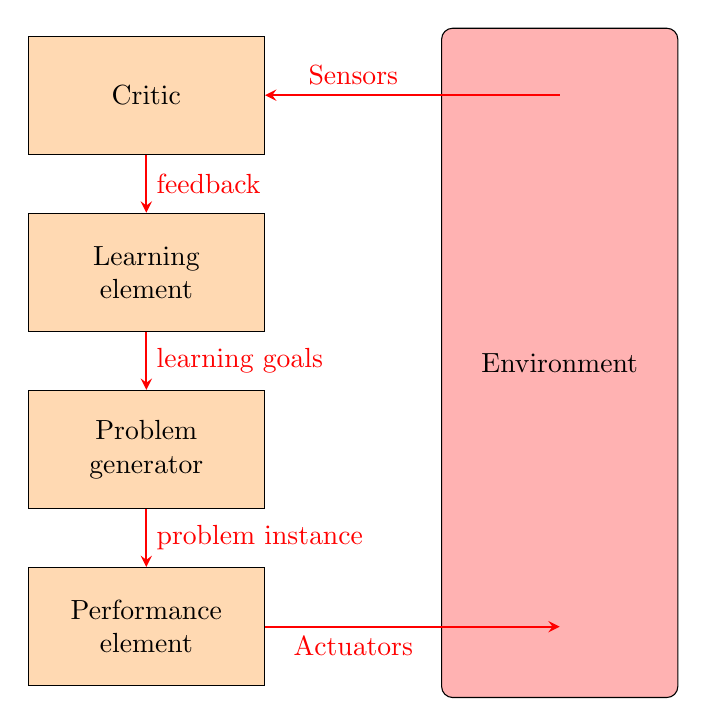
\begin{tikzpicture}[node distance=2.25cm]
        
        \node (critic) [ process] {Critic};
        \node (learning_element) [process, below of=critic] {Learning element};   
        \node (problem_generator) [process, below of=learning_element,] {Problem generator};   
        \node (performance_element) [process, below of=problem_generator,] {Performance element};   
        \node (environment) [environment, right of=critic, xshift=3cm, yshift=-3.4cm] {Environment};   
    
        \coordinate (B1) at ($ (environment) + (0,1)$);
        \coordinate (B2) at ($ (environment) - (0,1)$);
        \coordinate (perf_env) at ($ (environment)!(performance_element.east)!(B2) $);
        \coordinate (env_critic) at ($ (environment)!(critic.east)!(B1) $);

        \draw [arrow, red] (critic.south) -- node[anchor=west]{feedback} (learning_element.north);
        \draw [arrow, red] (learning_element.south) -- node[anchor=west, ]{learning goals} (problem_generator.north);
        \draw [arrow, red] (problem_generator.south) -- node[anchor=west, ]{problem instance} (performance_element.north);
        \draw [arrow, red] (performance_element.east) -- node[anchor=north, xshift=-0.75cm]{Actuators} (perf_env);
        \draw [arrow, red] (env_critic) -- node[anchor=south,xshift=-0.75cm]{Sensors} (critic.east);
        
        \end{tikzpicture}
    \end{minipage}
    ~\hspace{2cm}
    \begin{minipage}[c]{0.4\textwidth}
    
        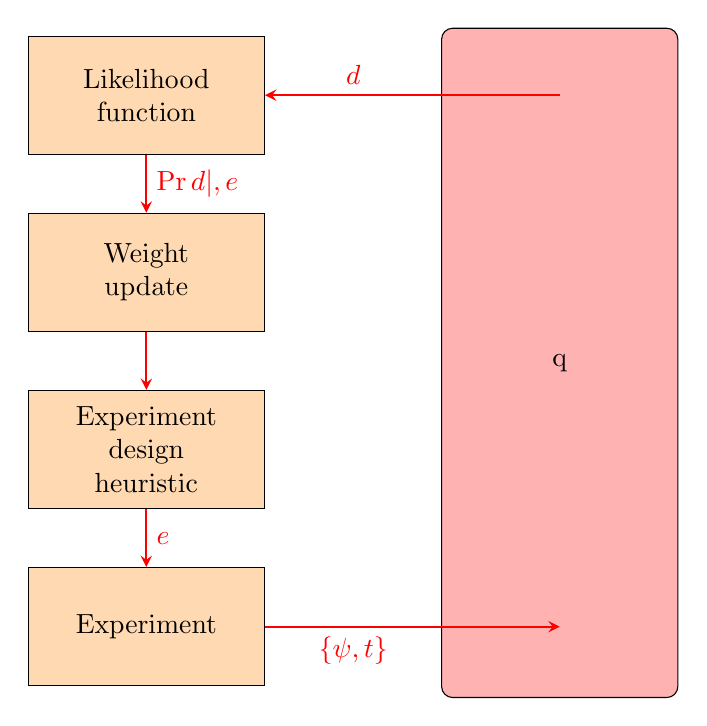
\begin{tikzpicture}[node distance=2.25cm]
        
        \node (critic) [ process] {Likelihood function};
        \node (learning_element) [process, below of=critic] {Weight update};   
        \node (problem_generator) [process, below of=learning_element,] {Experiment design heuristic};   
        \node (performance_element) [process, below of=problem_generator,] {Experiment};   
        \node (environment) [environment, right of=critic, xshift=3cm, yshift=-3.4cm] {\gls{q} };   
    
        \coordinate (B1) at ($ (environment) + (0,1)$);
        \coordinate (B2) at ($ (environment) - (0,1)$);
        \coordinate (perf_env) at ($ (environment)!(performance_element.east)!(B2) $);
        \coordinate (env_critic) at ($ (environment)!(critic.east)!(B1) $);

        \draw [arrow, red] (critic.south) -- node[anchor=west]{$\Pr\bk{d | \al, e}$} (learning_element.north);
        \draw [arrow, red] (learning_element.south) -- node[anchor=west, ]{$\pra$} (problem_generator.north);
        \draw [arrow, red] (problem_generator.south) -- node[anchor=west, ]{$e$} (performance_element.north);
        \draw [arrow, red] (performance_element.east) -- node[anchor=north, xshift=-0.75cm]{$\{ \ket{\psi}, t \}$} (perf_env);
        \draw [arrow, red] (env_critic) -- node[anchor=south,xshift=-0.75cm]{$d$} (critic.east);
        
        \end{tikzpicture}
    \end{minipage}


    \caption[Learning agents]{
        Learning agents. \textbf{Left,} definition of a learning agent, where an \emph{environment} is affected by 
        \emph{actuators} which realise a \emph{problem instance}, designed by a \emph{problem generator}, through some \emph{performance element}. 
        The result of the agent's action is detected by \emph{sensors}, which the \emph{critic} interprets with respect to
        the agent's \emph{learning goals}, by providing \emph{feedback} to the \emph{learning element}. 
        \textbf{Right,} mapping of the concept of a learning agent on to an individual model. 
        A target quantum system, \gls{q}, is queried by performing some \gls{experiment} $e$, 
        designed by an \acrlong{edh}, and implemented by evolving a \gls{probe} state $\ket{\psi}$ for time $t$. 
        The systems is measured, and the datum $d$ is sent to the  \gls{likelihood} function, which sends the \gls{likelihood} $\Pr(d|\al, t)$
        to the weight update (and the parameter distribution update), before designing another experiment. 
    }
    \label{fig:learning_agent}
\end{figure}

   